\chapter{About the Datasets used}
\ifpdf
    \graphicspath{{Chapter3/Chapter3Figs/PNG/}{Chapter3/Chapter3Figs/PDF/}{Chapter3/Chapter3Figs/}}
\else
    \graphicspath{{Chapter3/Chapter3Figs/EPS/}{Chapter3/Chapter3Figs/}}
\fi

\section{Calgary-Campinas Public MR dataset}\label{sec:3_1}
\markboth{\MakeUppercase{\thechapter. About the Datasets used}}{\thechapter. About the Datasets used}

\nomenclature[zT]{$T$}{Tesla (Measures Magnetic Field Strength)}

A collaborative effort between researchers at the Vascular Imaging Lab located at the University of Calgary and the Medical Image Computing Lab located at the University of Campinas (UNICAMP) resulted in the Calgary-Campinas Public MR dataset \cite{SOUZA2018482}.\\

The Calgary-Campinas Public MR dataset consists of 359 MRIs of healthy adults in the range of 29-80 years old. It consists of images from MRI scanners with two magnetic field strengths 1.5T (Tesla) and 3T (Tesla) and also contains scanners from 3 different companies, they are GE, Philips and Siemens. The data is also well divided among all the six combinations formed by the company name and magnetic field strength with approximately 60 images in each. The dataset is also gender and age-balanced as much as possible with the subjects at hand.\\

\begin{figure}[!htbp]
  \begin{center}
    \leavevmode
    \ifpdf
      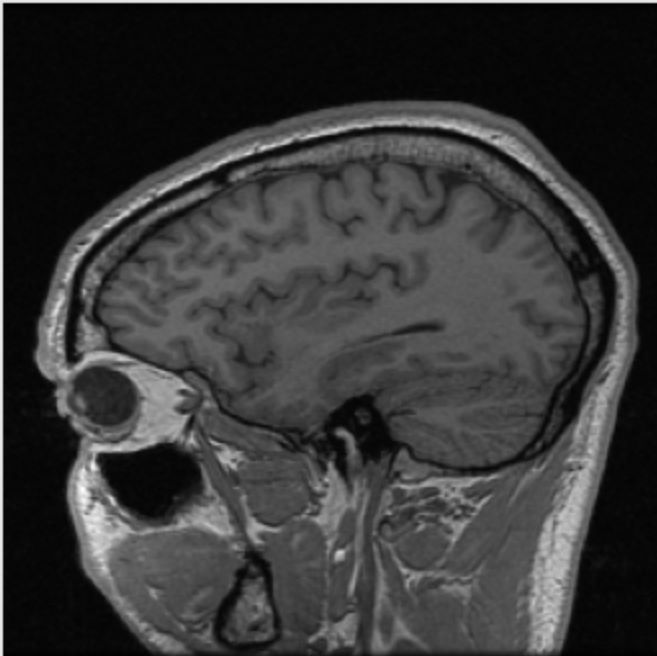
\includegraphics[height=3in]{Chapter3/Chapter3Figs/calgary_campinas_image.jpg}
    \else
      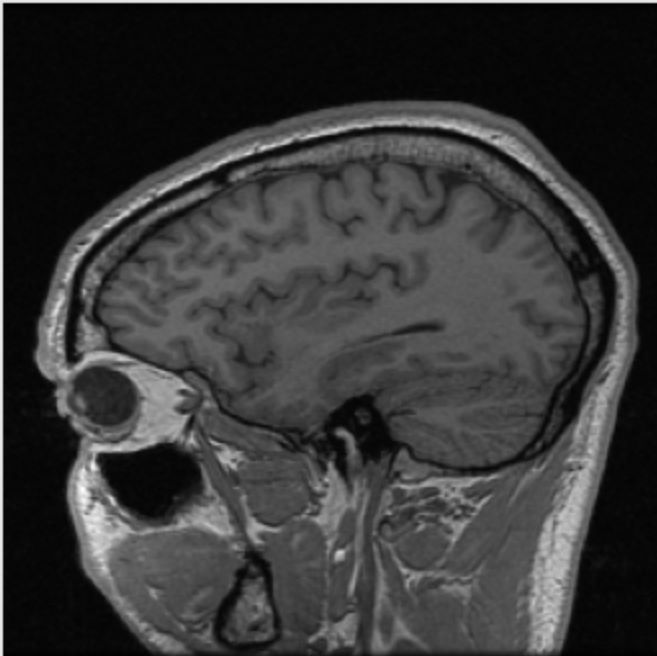
\includegraphics[bb = 92 86 545 742, height=3in]{Chapter3/Chapter3Figs/calgary_campinas_image.jpg}
    \fi
    \caption{Example MRI slice (image domain) from Calgary-Campinas dataset}
    \label{campinas1}
  \end{center}
\end{figure}

We have used 45 sideways brain MRIs from the Calgary-Campinas dataset (Single-channel coil data).\\

The MRIs have been divided into 25 for training (4524 slices), 10 for validation (1700 slices) and 10 for testing (1700 slices). Each MRI has approx 170 slices and the per-slice resolution is 256 X 256.\\

The purpose of using the single coil Calgary-Campinas dataset is to have a dataset that gives sharp images of healthy individuals and also is small enough to easily allow us to work with it, given the limited memory allocated to us on the provided hardware. The dataset was primarily used to train the W-Net, W-Net combined and W-Net 3-layer models, discussed in more detail in \ref{sec:prob_1}.\\

\section{fastMRI dataset}\label{sec:3_2}
\markboth{\MakeUppercase{\thechapter. About the Datasets used }}{\thechapter. About the Datasets used}

The fastMRI dataset \cite{zbontar2019fastmri} is a large-scale collection of both raw MR measurements and clinical MR images, that can be used for training and testing various machine learning approaches including MRI reconstruction, super-resolution, etc.\\

We used a small portion of the brain mulitcoil MRI scan data containing 10-30 slices in each MRI scan and with variable resolutions. We purposed the provided data to give us a fixed resolution of 248 X 248 while ensuring no loss of relevant data and managed to obtain 5473 slices, where 80\% was allotted to training and 20\% was allotted to validation with 50 remaining for training.\\

We used this data initially to train known models such as ESPCN and EDSR to study the existing SR (Super Resolution) models and have a perspective of their capabilities when working with MRIs and the problems that often appear with them.\\

\begin{figure}[!htbp]
  \begin{center}
    \leavevmode
    \ifpdf
      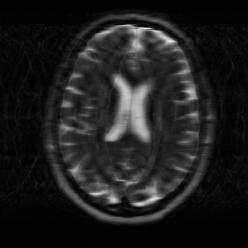
\includegraphics[height=3in]{Chapter3/Chapter3Figs/challenge_brain_Philips_6751018450_AXT2TSE_3_.png}
    \else
      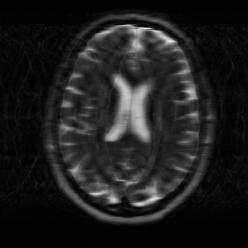
\includegraphics[bb = 92 86 545 742, height=3in]{Chapter3/Chapter3Figs/challenge_brain_Philips_6751018450_AXT2TSE_3_.png}
    \fi
    \caption{An example MRI used from the fastMRI dataset}
    \label{FigFmri}
  \end{center}
\end{figure}

\section{Brain Tumor Segmentation(BraTS2020) dataset}\label{sec:3_3}
\markboth{\MakeUppercase{\thechapter. About the Datasets used }}{\thechapter. About the Datasets used}

The Brain Tumor Segmentation(BraTS2020) dataset \cite{menze2015multimodal, bakas2017advancing, bakas2018identifying} includes pre-operative MRI scans of patients with various types of brain tumours and is often used for brain tumour segmentation and analysis.\\

One MRI scan in the dataset has four different MRI modalities, they are native (T1) scans, post-contrast T1-weighted, T2-weighted and T2-flair. These scans were sourced from many scanners from 19 institutions.\\

The dataset has been purposed to provide us with 3312 images of 512 X 512 MR images. Brain MRI data is preferred for comparison as compared to other regions because of the very fine details present in the brain MRIs along with minimal artefacts that come in especially handy when it comes to Super Resolution tasks.\\

We preferred this dataset over fMRI dataset \ref{sec:3_1} because we observed a ringing effect in the fMRI multicoil scans and hence didn't want to compromise the results of super-resolution because of those artefacts. Calgary-Campinas dataset \ref{sec:3_2} on the other hand works with healthy humans but instead we want the SR problem to focus on a real-world environment. The BraTS dataset provides us with brain tumour MRIs to ensure that the results we obtain are reproducible in a real-world environment for this specific problem. This is because SR is extremely sensitive to varied environments and hence we preferred this dataset for the SR problem.

\begin{figure}[!htbp]
  \begin{center}
    \leavevmode
    \ifpdf
      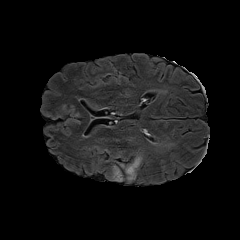
\includegraphics[height=3in]{Chapter3/Chapter3Figs/volume_12_slice_80.png}
    \else
      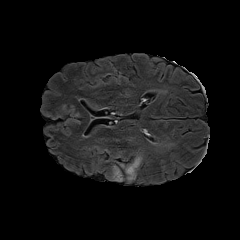
\includegraphics[bb = 92 86 545 742, height=3in]{Chapter3/Chapter3Figs/volume_12_slice_80.png}
    \fi
    \caption{An example MRI used from the BraTS 2020 dataset}
    \label{FigFmri}
  \end{center}
\end{figure}

% ------------------------------------------------------------------------


%%% Local Variables: 
%%% mode: latex
%%% TeX-master: "../thesis"
%%% End: 
